\documentclass[12pt,a4paper]{article}

% ============================================================
% PACKAGES
% ============================================================
\usepackage[utf8]{inputenc}
\usepackage[T1]{fontenc}
\usepackage{lmodern}
\usepackage[margin=2.5cm]{geometry}
\usepackage{amsmath,amssymb}
\usepackage{booktabs}
\usepackage{array}
\usepackage{longtable}
\usepackage{hyperref}
\usepackage{xcolor}
\usepackage{microtype}
\usepackage{parskip}
\usepackage{enumitem}
\usepackage{titlesec}
\usepackage{fancyhdr}
\usepackage{abstract}
\usepackage{authblk}
\usepackage{setspace}
\usepackage{tabularx}
\usepackage{multirow}
\usepackage{tikz}
\usetikzlibrary{arrows.meta, positioning, shapes.geometric}

% ============================================================
% HYPERREF SETUP
% ============================================================
\hypersetup{
  colorlinks=true,
  linkcolor=black,
  citecolor=black,
  urlcolor=blue,
  pdftitle={The Anti-Aging / Prion Coupling Topology},
  pdfauthor={Eric Robert Lawson},
}

% ============================================================
% HEADER / FOOTER
% ============================================================
\pagestyle{fancy}
\fancyhf{}
\rhead{\small OrganismCore --- Attractor Medicine Series}
\lhead{\small Lawson, E.R. (2026)}
\cfoot{\thepage}
\renewcommand{\headrulewidth}{0.4pt}

% ============================================================
% SECTION FORMATTING
% ============================================================
\titleformat{\section}{\large\bfseries\scshape}{}{0em}{}[\titlerule]
\titleformat{\subsection}{\normalsize\bfseries}{}{0em}{}
\titleformat{\subsubsection}{\normalsize\itshape}{}{0em}{}

% ============================================================
% CUSTOM COMMANDS
% ============================================================
\newcommand{\raging}{$R_{\mathrm{AGING}}$}
\newcommand{\rprion}{$R_{\mathrm{PRION}}$}
\newcommand{\prpc}{PrP$^{\mathrm{C}}$}
\newcommand{\prpsc}{PrP$^{\mathrm{Sc}}$}
\newcommand{\tpeold}{TPE-OLD}
\newcommand{\novel}[1]{\noindent\colorbox{yellow!18}{\parbox{\dimexpr\linewidth-2\fboxsep}{%
  \textbf{[NOVEL CLAIM:]} #1}}\vspace{0.4em}}
\newcommand{\confirmed}[1]{\noindent\colorbox{green!10}{\parbox{\dimexpr\linewidth-2\fboxsep}{%
  \textbf{[CONFIRMED:]} #1}}\vspace{0.4em}}
\newcommand{\Inet}[1]{$I_{#1}$}
\newcommand{\coupling}[2]{\medskip\noindent\rule{\linewidth}{0.4pt}\\
  \textbf{Coupling~#1} (#2)\\[0.3em]}

% ============================================================
% DOCUMENT
% ============================================================
\begin{document}

% ============================================================
% TITLE BLOCK
% ============================================================
\begin{titlepage}
\vspace*{1.5cm}
{\LARGE\bfseries The Anti-Aging / Prion Coupling Topology:\\[0.5em]
\large Intervention Graph Analysis, Equilibrium Waddington\\
Landscape Design, and the Six-Claim Novel Derivation\\
from the Identity Axis Framework}

\vspace{1.5em}

\author[1]{Eric Robert Lawson}
\affil[1]{OrganismCore (independent) --- ORCID: 0009-0002-0414-6544\\
\href{mailto:OrganismCore@proton.me}{OrganismCore@proton.me}}

\vspace{1.5em}

\noindent\textbf{Date:} 2026-03-09\\
\textbf{Status:} Active --- Speculative Derivation, Grounded.\\
\textbf{Trilogy position:} Paper~3 of~3 in the Aging--Prion--Coupling series.\\
\textbf{Framework DOI:}
\href{https://doi.org/10.5281/zenodo.18898788}{10.5281/zenodo.18898788}\\
\textbf{Paper~1 (Prion Diseases):}
\href{https://doi.org/10.5281/zenodo.18920269}{10.5281/zenodo.18920269}\\
\textbf{Repository:}
\href{https://github.com/Eric-Robert-Lawson/attractor-oncology}{github.com/Eric-Robert-Lawson/attractor-oncology}\\
\textbf{Source document:} \texttt{ANTI\_AGING\_PRION\_COUPLING\_EQUILIBRIUM\_DERIVATION.md}

\vspace{1.5em}
\noindent\rule{\textwidth}{0.8pt}

\begin{abstract}
\noindent
This paper derives a distinct and previously unnamed object of analysis:
the \textit{drug target interaction topology} of a combined anti-aging and
prion prophylaxis protocol. When the interventions derived from the Identity
Axis Framework are mapped as a seven-node graph (\Inet{1}--\Inet{7}), four
antagonistic couplings emerge that determine whether the combined protocol
is safe and whether it closes into a stable Waddington equilibrium or
amplifies the risks it is designed to prevent.

The four couplings and their resolutions are derived precisely:
(1)~\Inet{1}~$\to$~cancer: telomere maintenance supplies the same telomerase
mechanism used by 90\% of cancers; resolved by sequencing \Inet{7} before
\Inet{1}; (2)~\Inet{4}~$\dashv$~\Inet{7}: chronic mTOR suppression degrades
immune surveillance; resolved by pulsed scheduling with \Inet{5} covering the
autophagy gap; (3)~\Inet{5}~$\dashv$~neuroprotection: \prpc{} substrate
reduction removes normal copper-binding and NMDA-modulating functions;
resolved at 50--60\% partial dosing plus \Inet{6} synergy, with permanent
dissolution via G127V base editing; (4)~\Inet{2}~$\to$~transition-zone
instability: Identity Anchor agonism in Hub-locked cells creates
transcriptional conflict; resolved by mandatory Hub inhibitor
co-administration.

Cross-species validation shows that natural selection independently produced
three viable solutions to this same topology. The equilibrium Waddington
landscape is defined as the state in which every major identity drift
pathway is covered with two-node redundancy and all antagonistic edges are
mitigated. Six novel claims are locked with timestamp 2026-03-09, each
assigned a named falsifying experiment.
\end{abstract}

\noindent\rule{\textwidth}{0.8pt}
\end{titlepage}

% ============================================================
\tableofcontents
\newpage
% ============================================================

% ============================================================
\section{Preamble: What This Paper Is and Why It Exists}
% ============================================================

The previous two papers in this series established:

\begin{itemize}[leftmargin=2em]
  \item \textbf{Paper~1 (Prion Diseases,
    \href{https://doi.org/10.5281/zenodo.18920269}{DOI:10.5281/zenodo.18920269}):}
    Prion diseases are conformational false attractors in protein eigenfunction
    space (\rprion{} = energy barrier / templating efficiency). Drug targets:
    \Inet{5} PRNP-ASO (ION717), \Inet{6} anle138b, permanent dissolution via
    G127V base editing (Synthetic Fore Strategy).

  \item \textbf{Paper~2 (Aging):}
    Telomere shortening progressively withdraws \tpeold{} chromatin silencing,
    releasing aging drift genes (ISL2, VASP) that compete with Identity Anchor
    programmes. This is formalised as \raging{} $= A_{\mathrm{AGING}} /
    H_{\mathrm{drift}}$. Drug targets: \Inet{1} telomere maintenance,
    \Inet{2} Identity Anchor agonism, \Inet{3} aging drift gene silencing.
    Cancer surveillance (\Inet{7}) and autophagy maintenance (\Inet{4}) are
    shared nodes across both disease domains.
\end{itemize}

\textbf{The question this paper answers:} When all of these interventions are
applied simultaneously to a single human being, what happens? Do they reinforce
each other, or do they interfere? Is there a safe order? Is there an equilibrium?

The answer is not obvious. Several of the interventions target mechanisms that
the same biology uses for opposite purposes. This paper maps those conflicts
precisely, derives their resolutions, and specifies the topology of the
equilibrium state.

\begin{quote}
\textit{The drug target interaction topology is a distinct object of analysis
from any individual drug mechanism. The topology reveals what the individual
mechanisms do not: sequence constraints, redundancy requirements, coupling
risks, and dissolution strategies. No prior work has applied this analysis to
aging-cancer-prion coupled intervention design.}
\end{quote}

% ============================================================
\section{Part~I: The Seven-Node Intervention Graph}
% ============================================================

\subsection{Node Definitions}

\begin{longtable}{p{1.2cm} p{3cm} p{4cm} p{4cm}}
  \toprule
  \textbf{Node} & \textbf{Name} & \textbf{Mechanism} & \textbf{Primary
  target disease} \\
  \midrule
  \Inet{1} & Telomere maintenance & Telomere length preservation;
    telomerase activity in somatic tissue & Aging (\tpeold{} drift
    prevention) \\
  \addlinespace
  \Inet{2} & Identity Anchor agonism & dCas9-VP64 at $A$ loci; mRNA-LNP
    Identity Anchor delivery & Aging prevention; cancer Tier~2A \\
  \addlinespace
  \Inet{3} & Aging drift gene silencing & dCas9-EHMT2 targeted H3K9me3
    restoration at \tpeold{}-released loci (ISL2, VASP) & Aging
    (\raging{} maintenance) \\
  \addlinespace
  \Inet{4} & mTOR inhibition / autophagy & Rapamycin axis; autophagy
    induction; misfolded protein clearance & Prion; AD; PD; aging
    proteostasis \\
  \addlinespace
  \Inet{5} & PrP substrate reduction & PRNP-ASO (ION717); reduces \prpc{}
    expression to limit \prpsc{} templating substrate & Prion disease \\
  \addlinespace
  \Inet{6} & PrP conformation stabilisation & Anle138b; pharmacological
    chaperone raises energy barrier of \prpc{} against misfolding &
    Prion; AD ($\tau$); PD ($\alpha$-syn) \\
  \addlinespace
  \Inet{7} & Cancer surveillance (SSDD) & Immune surveillance
    enhancement; synthetic Spalax IFN-$\beta$ circuit detecting \raging{}
    below cancer threshold & Cancer \\
  \bottomrule
  \caption{The seven intervention nodes: names, mechanisms, and primary
    disease targets. Nodes \Inet{4}, \Inet{6}, and \Inet{7} are
    cross-cutting: they serve multiple disease domains simultaneously.}
\end{longtable}

\subsection{The Topology Diagram}

\begin{center}
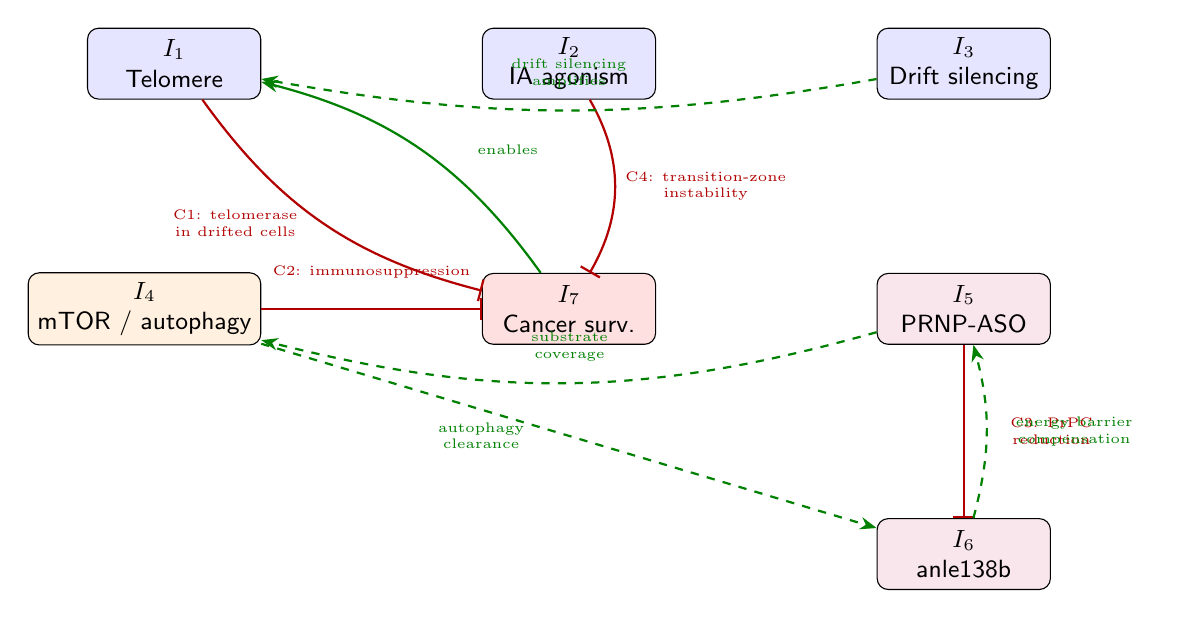
\begin{tikzpicture}[
  node distance=2.4cm and 2.8cm,
  every node/.style={draw, rounded corners, minimum width=2.2cm,
    minimum height=0.9cm, font=\small\sffamily, align=center},
  arrow/.style={-{Stealth[length=6pt]}, thick},
  inhibit/.style={-{Bar[width=8pt]}, thick, red!70!black},
  synergy/.style={-{Stealth[length=6pt]}, thick, green!50!black, dashed},
]
  % Nodes — two rows
  \node (I1) [fill=blue!10]  {\Inet{1}\\Telomere};
  \node (I2) [fill=blue!10, right=of I1]  {\Inet{2}\\IA agonism};
  \node (I3) [fill=blue!10, right=of I2]  {\Inet{3}\\Drift silencing};
  \node (I7) [fill=red!12, below=2.2cm of I2]   {\Inet{7}\\Cancer surv.};
  \node (I4) [fill=orange!12, left=of I7]  {\Inet{4}\\mTOR / autophagy};
  \node (I5) [fill=purple!10, right=of I7] {\Inet{5}\\PRNP-ASO};
  \node (I6) [fill=purple!10, below=2.2cm of I5]  {\Inet{6}\\anle138b};

  % Coupling 1: I1 -> cancer (needs I7 first)
  \draw[inhibit] (I1) to[bend right=20]
    node[midway, left, draw=none, font=\tiny, red!70!black]
    {C1: telomerase\\in drifted cells} (I7);

  % I7 enables I1 (conditional arrow)
  \draw[arrow, green!50!black] (I7) to[bend right=20]
    node[midway, right, draw=none, font=\tiny, green!50!black]
    {enables} (I1);

  % Coupling 2: I4 -| I7
  \draw[inhibit] (I4) --
    node[midway, above, draw=none, font=\tiny, red!70!black]
    {C2: immunosuppression} (I7);

  % I5 covers I4 gap
  \draw[synergy] (I5) to[bend left=15]
    node[midway, above, draw=none, font=\tiny, green!50!black]
    {substrate\\coverage} (I4);

  % Coupling 3: I5 -| neuroprotection
  \draw[inhibit] (I5) --
    node[midway, right, draw=none, font=\tiny, red!70!black]
    {C3: PrPC\\reduction} (I6);

  % I6 compensates I5
  \draw[synergy] (I6) to[bend right=15]
    node[midway, right, draw=none, font=\tiny, green!50!black]
    {energy barrier\\compensation} (I5);

  % Coupling 4: I2 -> instability (needs Hub inhibitor)
  \draw[inhibit] (I2) to[bend left=30]
    node[midway, right, draw=none, font=\tiny, red!70!black]
    {C4: transition-zone\\instability} (I7);

  % I3 supports I1
  \draw[synergy] (I3) to[bend left=10]
    node[midway, above, draw=none, font=\tiny, green!50!black]
    {drift silencing\\amplifies} (I1);

  % I4 cross-action on I6 targets
  \draw[synergy] (I4) -- node[midway, left, draw=none, font=\tiny,
    green!50!black] {autophagy\\clearance} (I6);

\end{tikzpicture}
\end{center}

\vspace{0.5em}
\noindent\textit{Red barred arrows = antagonistic couplings. Green dashed
arrows = synergistic / enabling relationships. Blue nodes = aging arm.
Orange node = shared proteostasis. Purple nodes = prion arm.
Red node = keystone (I7).}

% ============================================================
\section{Part~II: The Four Antagonistic Couplings}
% ============================================================

\subsection{Coupling~1: \texorpdfstring{\Inet{1}~$\to$~Cancer}{I1 -> Cancer}}

\coupling{1}{\Inet{1} (telomere maintenance) $\to$ cancer risk amplification}

\textbf{The mechanism of conflict:}

Telomere maintenance (\Inet{1}) raises \raging{} by preventing \tpeold{}
drift --- which is exactly the desired effect. However, the mechanism of
telomere lengthening is telomerase activation in somatic tissue. Telomerase
activation in somatic cells is the same mechanism by which approximately 90\%
of all cancers achieve replicative immortality (TERT upregulation via promoter
mutation or amplification).

Activating TERT for anti-aging in normal committed cells provides the same
replicative immortality signal to any cell that has \textit{already} begun to
drift toward a false attractor. If that cell is in the early drift zone
(\raging{} falling but Hub not yet locked), telomere maintenance is
beneficial: it raises \raging{} back toward the normal range. If that cell has
\textit{already} crossed the cancer activation energy threshold, telomere
maintenance in that cell is oncogenic.

\confirmed{Telomerase activation is a confirmed oncogenic mechanism in
$\sim$90\% of cancers. TERT promoter mutation is the most commonly recurring
non-coding mutation in cancer (Bladder SCC, melanoma, glioblastoma, HCC, and
others). Greider and Blackburn 1985; Shay and Wright 2000.}

\textbf{The resolution:}

The coupling is resolved by \textbf{sequencing}. \Inet{7} (cancer surveillance /
SSDD) must be active and validated before \Inet{1} is applied.

\begin{quote}
\textbf{Protocol rule:} Establish \Inet{7}. Clear all cells with
\raging{} below the cancer threshold. Confirm surveillance is operational.
\textit{Then} activate \Inet{1} in a confirmed-clean cell population.
\Inet{7}~$\to$~\Inet{1}. Not \Inet{1} alone.
\end{quote}

If \Inet{1} is applied without \Inet{7}: telomere maintenance in cells
already at the false attractor threshold $\to$ those cells are immortalised
$\to$ cancer.

If \Inet{7} is applied before \Inet{1}: clean baseline. Surveillance active.
Then maintenance. The conditional edge is resolved by order of operations.

\textbf{The natural validation:}

The naked mole rat (NMR) runs constitutive somatic telomerase (\Inet{1}
always active) without cancer. The resolution: NMR simultaneously runs
permanent Tier~3 HMM-HA hypersensitive contact inhibition --- the
\Inet{7}-equivalent operating extracellularly, continuously, unconditionally.
NMR does not \textit{activate} surveillance when needed. It \textit{never
turns it off}. The conditional edge (\Inet{1} conditional on \Inet{7}) is
unconditionally satisfied by the NMR's structural topology.

The elephant solution is the opposite: maximum \Inet{7} (TP53~$\times$20,
every damaged cell undergoes immediate decisive apoptosis) with minimal
\Inet{1}. Zero cancer but conservative tissue regeneration.

\novel{Patients receiving anti-aging telomere maintenance therapies
\textit{without} robust cancer surveillance will show elevated cancer
incidence disproportionate to the expected effect of telomere lengthening
alone. The topological analysis predicts this clinical signal before any
trial has produced it. TEST: Prospective cohort study tracking cancer
incidence in participants receiving TERT-activating compounds stratified by
whether cancer surveillance biomarker panel (\raging{} = $A_{\mathrm{AGING}}
/ H_{\mathrm{drift}}$) is co-monitored. Primary endpoint: false attractor
formation rate.}

\subsection{Coupling~2: \texorpdfstring{\Inet{4}~$\dashv$~\Inet{7}}{I4 -| I7}}

\coupling{2}{\Inet{4} (mTOR inhibition / rapamycin) $\dashv$ cancer immune
surveillance (\Inet{7})}

\textbf{The mechanism of conflict:}

mTOR inhibition (\Inet{4}) activates autophagy, which clears \prpsc{},
$\tau$, and $\alpha$-synuclein aggregates --- a direct anti-prion, anti-AD,
and anti-PD mechanism. mTOR inhibition also extends lifespan in mammals.
Both effects are confirmed.

However: mTOR is a critical regulator of lymphocyte proliferation and NK
cell activation. Chronic mTOR suppression is the reason rapamycin is used
clinically as an immunosuppressant in transplant medicine. The immune cells
whose proliferation is suppressed are the same immune cells that execute the
cancer surveillance function of \Inet{7}. Chronic \Inet{4} undermines chronic
\Inet{7}.

\confirmed{Rapamycin is an FDA-approved immunosuppressant. Long-term rapamycin
users show elevated susceptibility to opportunistic infections. T-cell
proliferation and NK cell activation are both mTOR-dependent. This is not
hypothetical. Kennedy and Lamming 2016.}

\textbf{The resolution:}

\textbf{Pulsed rather than continuous} mTOR inhibition. A cyclical dosing
schedule (e.g., once weekly --- confirmed to extend lifespan in mice with
substantially reduced immunosuppression relative to daily dosing) allows
autophagy induction to occur during the dosing period while immune function
recovers in the gap.

The critical insight is that the two effects have different kinetic profiles:
autophagy induction by rapamycin persists for 48--72 hours after a single
dose, while T-cell proliferation capacity recovers within 3--5 days of
dose interruption. The pulsed schedule can be designed so the clearance
effect is captured while the immune effect is not chronically suppressed.

\textbf{Redundancy coverage:} \Inet{5} (PRNP-ASO) provides a
\textit{substrate-level} prion defence that does not depend on autophagy or
immune function. If \Inet{4} is pulsed (reduced autophagy clearance between
doses), \Inet{5} ensures that \prpc{} substrate is not available for
\prpsc{} templating. \Inet{4} and \Inet{5} are redundant nodes in the prion
defence subgraph --- different mechanisms, same target. Pulsing \Inet{4} does
not create a prion vulnerability window because \Inet{5} covers that window.

\novel{The optimal rapamycin pulse schedule for the combined protocol differs
from the optimal schedule for either anti-aging or anti-prion application
alone. The combined protocol requires a dosing interval that preserves
\Inet{7} immune competence beyond what is needed for isolated longevity
benefit. TEST: Comparative NK cell and T-cell functional assay in aged mice
receiving (a) continuous rapamycin, (b) once-weekly rapamycin, (c) pulsed
rapamycin + PRNP-ASO. Endpoint: cancer surveillance capacity + prion
propagation rate per condition.}

\subsection{Coupling~3: \texorpdfstring{\Inet{5}~$\dashv$~Neuroprotection}{I5 -| Neuroprotection}
--- The Deepest Coupling}

\coupling{3}{\Inet{5} (PRNP-ASO, \prpc{} substrate reduction)
$\dashv$ neuronal oxidative stress resistance and NMDA protection}

\textbf{The mechanism of conflict:}

\prpc{} has confirmed normal physiological functions in neurons:
copper binding and antioxidant defence at synapses; NMDA receptor modulation
(prevention of excitotoxicity); neurite outgrowth and synaptogenesis;
neuroprotection from oxidative stress. These functions are established in
PrP-knockout mouse models, which are viable under standard conditions but
significantly more vulnerable to oxidative stress challenge, seizure, and
excitotoxic insult than wild-type controls.

\Inet{5} reduces \prpc{} expression to limit \prpsc{} propagation. At the
80\% reduction level required for maximal prion protection, these
neuroprotective functions are reduced by approximately 80\%.

\begin{quote}
\textbf{The structural form of Coupling~3:} This is the textbook definition
of \textit{antagonistic pleiotropy at the protein level}. The same molecule
whose \textit{presence} prevents one failure (neuronal identity drift from
oxidative damage --- Level~1 identity failure) and whose \textit{absence}
prevents another (prion propagation --- Level~4 identity failure) exists in
a two-sided trade-off that cannot be resolved by dose alone when the goal is
maximum protection from both failures simultaneously.
\end{quote}

\confirmed{PrP-knockout mice show significantly elevated neuronal
vulnerability to oxidative stress, kainate-induced seizures, and excitotoxic
challenge compared to wild-type. Copper-binding function of \prpc{} at the
synapse is confirmed. NMDA receptor modulation by \prpc{} is confirmed.
Watt et al.\ 2012; Khosravani et al.\ 2008.}

\textbf{The resolution --- three tiers:}

\begin{description}[leftmargin=2em, itemsep=0.5em]
  \item[\textbf{Tier~A --- Partial dosing (50--60\%):}]
    At 50--60\% \prpc{} reduction, published data shows significant and
    clinically meaningful prion survival benefit (not as large as 80\% but
    sufficient). Residual 40--50\% \prpc{} maintains copper-binding
    capacity, NMDA modulation, and antioxidant function. This is the
    \textit{titration equilibrium}: the dose that minimises both risks
    simultaneously.

  \item[\textbf{Tier~B --- \Inet{6} synergy:}]
    Anle138b (\Inet{6}) raises the energy barrier of the
    \textit{remaining} \prpc{} against misfolding. Combined effect: 50\%
    reduction of substrate (\Inet{5}) + raised energy barrier of remaining
    substrate (\Inet{6}). The net effective conversion rate is equivalent to
    80--90\% substrate reduction without the neuroprotective deficit. \Inet{5}
    and \Inet{6} are \textit{synergistic} nodes in the prion defence
    subgraph: their combined effect exceeds what either achieves alone at
    safe doses.

  \item[\textbf{Tier~C --- G127V base editing (Synthetic Fore Strategy,
    permanent dissolution):}]
    The Coupling~3 trade-off arises because reducing \prpc{}
    \textit{quantity} simultaneously removes its protective and
    risk-generating functions. If instead \prpc{} \textit{sequence} is
    changed to G127V, the protein retains all neuroprotective functions
    (copper binding, NMDA modulation, synaptogenesis) while acquiring
    energy-barrier residues that make it completely resistant to \prpsc{}
    templating. High \prpc{} expression no longer creates prion risk because
    the protein cannot occupy the false attractor conformation.

    The coupling is not managed --- it is \textit{dissolved}. The
    neuroprotective function is preserved. The templating substrate is
    eliminated. Two distinct properties of the same protein are separated
    by changing a single codon.

    This is what the Fore people's evolution produced over four generations
    in response to lethal kuru prion pressure. The framework identifies it
    not as an interesting anthropological observation but as a
    proof-of-concept that permanent coupling dissolution is biologically
    achievable.
\end{description}

\novel{G127V base-edited neurons will show PrP$^{\mathrm{C}}$ neuroprotective
function \textit{indistinguishable} from wild-type G127 neurons under
oxidative stress and excitotoxic challenge, while showing complete resistance
to \prpsc{} seeding. This is the desired outcome: it would confirm that the
coupling is dissolved rather than managed. TEST: Base editor delivery to
human iPSC-derived neurons. Challenge with (a)~\prpsc{} seeding, (b)~kainate
excitotoxicity, (c)~$H_2O_2$ oxidative stress. Compare G127V vs.\ wild-type
vs.\ PRNP-KO for both endpoints simultaneously.}

\subsection{Coupling~4: \texorpdfstring{\Inet{2}~$\to$~Transition-Zone Instability}{I2 -> Transition-Zone Instability}}

\coupling{4}{\Inet{2} (Identity Anchor agonism) $\to$ genomic
instability in Hub-locked cells}

\textbf{The mechanism of conflict:}

Identity Anchor agonism (\Inet{2}) --- restoring or amplifying the cell-type
specific Identity Anchor transcription factor programme --- is the framework's
Tier~2A drug logic in every cancer derivation. In the aging prevention context,
it is applied to cells that are in the \textit{aging drift zone}: \raging{}
falling but the convergence Hub not yet fully locked. At this stage, there is
no deep false attractor competing with the correct identity programme. \Inet{2}
is safe and effective here.

The conflict arises if \Inet{2} is applied to a cell that has \textit{already}
Hub-locked into a deep false attractor (\raging{} near zero). In that cell,
the restored Identity Anchor signal competes with the already-locked Hub. The
cell receives two simultaneous strong signals: the correct identity from
\Inet{2}, and the false attractor from the active Hub. This creates
transcriptional instability --- the cell oscillates between two attractor
basins and accumulates genomic errors at an elevated rate. The framework calls
this the \textit{transition zone}: the instability belt between two attractors.

\textbf{The resolution:}

\Inet{2} must be combined with a Hub inhibitor (Tier~2 in the framework) as
a combined treatment. The Hub must be reduced \textit{before or simultaneously}
with Identity Anchor agonism. Then \Inet{2} has a clear return path (the
correct attractor) without Hub competition.

\begin{quote}
\textbf{Mandatory protocol rule:} Never apply \Inet{2} alone in cells
confirmed to have Hub locking. \Inet{7} (surveillance) first identifies
Hub-locked cells. Hub inhibitor (Tier~2, disease-specific) reduces the
Hub. Then \Inet{2} restores the correct attractor. Three-step sequence:
\Inet{7}~$\to$~Hub inhibitor~$\to$~\Inet{2}. Not \Inet{2} alone.
\end{quote}

\textbf{In the aging prevention context specifically:} \Inet{2} is being
applied to cells in the drift zone, not the locked zone. The risk is lower.
But the stage-specific application is mandatory: the same drug, applied to
the same cell type at an earlier vs.\ later disease stage, has a different
risk profile. Stage-specific application of \Inet{2} is not optional.

% ============================================================
\section{Part~III: What Natural Selection Built --- Cross-Species
Topology Validation}
% ============================================================

\subsection{Overview}

The coupling problem described in Part~II is not a problem unique to
deliberate human intervention. Evolution has imposed exactly these coupling
pressures on every long-lived organism: maintaining genome integrity over
decades while preventing both cancer and neurodegeneration, in a body where
the tools for preventing one can accelerate the other. Natural selection
solved it, repeatedly and independently, using different node combinations.

Reading the cross-species data as topology validation reveals three
qualitatively distinct solutions that are all viable, and one coupling-
dissolution event that proves permanent resolution is achievable.

\subsection{Naked Mole Rat: The NMR Template --- Recommended for Human Intervention}

\begin{description}[leftmargin=2em]
  \item[\Inet{1} (telomere):] \textbf{SOLVED.} NMR telomeres do not shorten.
    Constitutively active somatic telomerase, unusual among mammals.
    
    \confirmed{Seluanov et al.\ 2013; Gorbunova et al.\ 2014.}

  \item[\Inet{7} (cancer surveillance):] \textbf{SOLVED at Tier~3.} HMM-HA
    hypersensitive contact inhibition operates extracellularly, continuously,
    before any cell can form a deep false attractor. The \Inet{7}-equivalent
    is never deactivated.
    
    \confirmed{Tian et al.\ 2013; Seluanov 2009.}

  \item[\Inet{4} (proteostasis):] \textbf{CONSTITUTIVELY UPREGULATED.}
    NMR proteasome is more active and more robust than mouse or human.
    Autophagy baseline is elevated. Spontaneous \prpsc{} events are cleared
    before propagation. NMR may have solved the prion problem via \Inet{4}
    rather than \Inet{5}/\Inet{6}.
    
    \confirmed{Azpurua et al.\ 2013.}

  \item[\Inet{5}/\Inet{6} (prion sequence):] \textbf{OPEN QUESTION.}
    NMR PRNP sequence has not been studied for D163/G127V-equivalent
    protective residues. The framework predicts: either NMR has protective
    \prpc{} residues OR the constitutive \Inet{4} proteostasis is sufficient.
\end{description}

\textbf{Topology solution:} The NMR solved the \Inet{1}~$\to$~cancer coupling
(Coupling~1) by making \Inet{7} \textit{unconditionally active} rather than
conditionally activated. The conditional edge (\Inet{1} requires \Inet{7})
is satisfied permanently by structural means. This is the optimal topology
for human intervention because it achieves maximum longevity (\Inet{1} always
active) without sacrificing tissue regeneration capacity (unlike the elephant
solution below).

\novel{NMR PRNP sequence analysis will reveal either (a) protective residues
equivalent to D163/G127V, confirming structural prion resistance, or (b)
wild-type susceptible sequence, in which case the NMR proteostasis (\Inet{4})
must be sufficient to prevent spontaneous \prpsc{} propagation in the
35--40-year NMR lifespan. These are mutually exclusive outcomes, both
testable, and both informative for the human topology design.}

\subsection{Bowhead Whale: Enhanced DNA Repair Topology}

The bowhead whale (\textit{Balaena mysticetus}, 200+ year lifespan,
80,000~kg body mass) represents a second viable topology:

\begin{description}[leftmargin=2em]
  \item[\Inet{7} (cancer surveillance):] \textbf{SOLVED at Tier~2B/DNA level.}
    Not via extra TP53 copies (that is the elephant strategy). Bowhead whales
    have evolved enhanced ERCC family DNA repair proteins, PCNA variants, and
    $>$500 cancer-resistance gene variants. Their cells catch damage at the
    DNA level before it becomes an oncogenic driver.
    \confirmed{Keane et al.\ 2015.}

  \item[\Inet{1} (telomere):] \textbf{IMPLIED.} A 200-year lifespan requires
    either non-shortening telomeres or extraordinary initial telomere length.
    Mechanism not fully characterised but the phenotype is confirmed.

  \item[\Inet{4} (proteostasis):] \textbf{CONSTITUTIVELY UPREGULATED.}
    200-year-old whale brains do not accumulate AD-type amyloid or prion
    aggregates at rates expected from human equivalents. Enhanced baseline
    proteostasis is the whale's \Inet{4}-equivalent defence.
\end{description}

\textbf{Topology solution:} Three nodes (\Inet{7}~+~\Inet{1}~+~\Inet{4}),
all constitutively active. No antagonistic couplings because \Inet{7} is
always running. Same structural logic as NMR but implemented through different
molecular means (DNA repair enhancement vs.\ extracellular matrix signalling).

\subsection{Elephant: Maximum \texorpdfstring{\Inet{7}}{I7}, Minimal
\texorpdfstring{\Inet{1}}{I1}}

The African elephant (5,000~kg, 70-year lifespan) runs a qualitatively
different topology:

\begin{description}[leftmargin=2em]
  \item[\Inet{7} (cancer surveillance):] \textbf{MAXIMUM AGGRESSION.}
    20 functional TP53 copies (19 retrogenes). Any cell with DNA damage
    undergoes immediate, decisive apoptosis. The cancer surveillance is
    hair-trigger: no cell gets a second chance to form a false attractor.
    \confirmed{Abegglen et al.\ 2015; Sulak et al.\ 2016.}

  \item[\Inet{1} (telomere):] \textbf{LIKELY MINIMAL.} Hyper-vigilant
    \Inet{7} would eliminate any cell receiving an anomalous proliferative
    signal as a potential false attractor. Constitutive telomerase in
    elephant somatic tissue is probably counter-productive for the elephant
    topology. Elephants likely accept the regenerative cost.
\end{description}

\textbf{Topology solution:} Maximum \Inet{7}, minimal \Inet{1}. The trade-off:
zero cancer, but conservative tissue regeneration (slower wound healing,
lower stem cell proliferative capacity). For human quality of life over a
200+ year lifespan, the NMR solution is superior: maximum \Inet{1} and
maximum \Inet{7}, achieved by structural rather than trigger-based \Inet{7}.

\subsection{The Fore People: Coupling Dissolution as Evolution}

The Fore people of Papua New Guinea experienced lethal kuru prion epidemic
pressure beginning in the early 20th century (and by historical analogy
earlier). Within four generations, a protective variant --- G127V in PRNP
--- swept to high frequency in exposed populations.

\begin{quote}
\textit{The Fore people's evolution is the only known case of natural
selection producing coupling dissolution in a human population. They did not
develop a more effective autophagy system (\Inet{4}) or a better molecular
chaperone (\Inet{6}). They eliminated the Coupling~3 trade-off by changing
the protein sequence so that the trade-off ceased to exist. G127V \prpc{}
binds copper, modulates NMDA receptors, and promotes synaptogenesis. It does
not template \prpsc{}.}
\end{quote}

\confirmed{G127V confers complete resistance to all known prion strains in
transgenic mouse models. Homozygous G127V individuals show no phenotypic
abnormality. Asante et al.\ 2015 (\textit{NEJM}).}

The framework reads this as a proof of concept: coupling dissolution is not
a theoretical possibility. It is a biological event that occurred in a human
population over a medically observable timescale. Base editing G127V into
human somatic cells is not speculation about a new protein engineering
challenge. It is a request to replicate a variant that human evolution has
already safety-tested over four generations.

% ============================================================
\section{Part~IV: The Redundant Subgraph Architecture}
% ============================================================

\subsection{Three Redundant Subgraphs}

The topology analysis reveals that the seven nodes naturally partition into
three redundant coverage subgraphs, each targeting the same disease domain
through multiple independent mechanisms:

\begin{longtable}{p{3cm} p{3.5cm} p{2.5cm} p{3.5cm}}
  \toprule
  \textbf{Subgraph} & \textbf{Nodes} & \textbf{Redundancy} &
  \textbf{Coverage} \\
  \midrule
  Prion defence subgraph &
    \Inet{4} + \Inet{5} + \Inet{6} &
    3-node, 3 mechanisms &
    Autophagy clearance + substrate reduction + energy barrier
    raising \\
  \addlinespace
  Aging drift prevention subgraph &
    \Inet{1} + \Inet{2} + \Inet{3} &
    3-node, 3 mechanisms &
    Telomere maintenance + Identity Anchor agonism + drift gene
    silencing \\
  \addlinespace
  Cancer surveillance subgraph &
    \Inet{7} + \Inet{3} + \Inet{1} &
    3-node, 3 levels &
    Surveillance (cellular) + drift prevention (epigenetic) +
    valley maintenance (telomere) \\
  \bottomrule
  \caption{The three redundant subgraphs. The cancer subgraph notably
    includes \Inet{1} and \Inet{3} from the aging arm: the same
    interventions that prevent aging drift are the first lines of cancer
    prevention.}
\end{longtable}

\textbf{The two keystone cross-cutting nodes:}

\begin{description}[leftmargin=2em]
  \item[\textbf{\Inet{6} (anle138b):}] Crosses between all three Level~4
    propagating protein entries simultaneously. Anle138b has confirmed
    preclinical activity against \prpsc{} (prion), $\alpha$-synuclein
    (PD), and $\tau$ (AD) aggregation through the same aggregate-interface
    stabilisation mechanism. One compound providing \Inet{6}-level defence
    across three disease categories.

  \item[\textbf{\Inet{7} (cancer surveillance):}] Is simultaneously the
    keystone for \Inet{1} (as established in Coupling~1) and the disease-
    specific Hub inhibitor platform for cancer-stage cells. It serves as
    both a prerequisite for the aging arm and an active therapeutic in the
    cancer arm.
\end{description}

% ============================================================
\section{Part~V: The Equilibrium Waddington Landscape}
% ============================================================

\subsection{Definition of the Equilibrium State}

The equilibrium Waddington landscape is defined as:

\begin{quote}
\textbf{A state in which every major false attractor formation pathway is
blocked by at least one active intervention AND in which no intervention
creates a new false attractor pathway that is not covered by another
intervention. No single node is a single point of failure. The topology has
redundancy at every critical node. All antagonistic edges are mitigated by
scheduling or dose titration.}
\end{quote}

\subsection{The Four Pathway Coverages}

\begin{longtable}{p{3.5cm} p{4cm} p{5cm}}
  \toprule
  \textbf{Disease pathway} & \textbf{Covering nodes} &
  \textbf{Redundancy architecture} \\
  \midrule
  Cancer / false attractor locking &
    \Inet{7} + \Inet{3} + \Inet{1} &
    Surveillance (cellular detection) + drift prevention (epigenetic
    maintenance) + valley maintenance (telomere length). Three
    independent mechanisms. \\
  \addlinespace
  Prion propagation &
    \Inet{5} + \Inet{6} + \Inet{4} &
    Substrate reduction + energy barrier + autophagy clearance. Long-
    term: G127V base editing replaces \Inet{5} permanently (dissolution).\\
  \addlinespace
  Neurodegeneration &
    \Inet{4} + \Inet{6} + \Inet{2} &
    Autophagy clears $\tau$, $\alpha$-syn, \prpsc{}. Anle138b active
    against all three targets. Identity Anchor agonism for MEF2C/NURR1 in
    neurons. Disease-specific Hub inhibitors (DYRK1A for AD, HDAC4/5 for
    PD) provide Tier~2. \\
  \addlinespace
  Aging drift (\tpeold{}) &
    \Inet{1} + \Inet{2} + \Inet{3} &
    Telomere length maintenance + Identity Anchor programme agonism +
    targeted silencing of drift-released genes. Three-node redundant
    system. \\
  \bottomrule
  \caption{The four major false attractor pathways and their redundant
    coverage in the equilibrium state.}
\end{longtable}

\subsection{The Resolved Antagonistic Edge Summary}

\begin{longtable}{p{3cm} p{3cm} p{6.5cm}}
  \toprule
  \textbf{Coupling} & \textbf{Type} & \textbf{Resolution} \\
  \midrule
  \Inet{1}~$\to$~cancer & Sequencing & \Inet{7} must precede \Inet{1}.
    NMR template: \Inet{7} structural and permanent (HMM-HA). \\
  \addlinespace
  \Inet{4}~$\dashv$~\Inet{7} & Scheduling & Pulsed rapamycin (e.g., weekly)
    preserves immune function recovery. \Inet{5} covers prion window. \\
  \addlinespace
  \Inet{5}~$\dashv$~neuroprotection & Partial dosing + synergy +
    dissolution & 50-60\% dosing + \Inet{6} synergy (short-term). G127V
    base editing dissolves the coupling permanently (long-term). \\
  \addlinespace
  \Inet{2}~$\to$~instability & Stage-gating + co-administration & Only
    in drift-zone cells (aging context). In cancer context: Hub inhibitor
    must precede or accompany \Inet{2}. \\
  \bottomrule
  \caption{Summary of the four antagonistic couplings and their resolutions.}
\end{longtable}

\subsection{The Equilibrium Is Dynamic, Not Static}

The equilibrium is not a one-time event. It is a dynamic steady state that
requires continuous maintenance:

\begin{itemize}[leftmargin=2em]
  \item \Inet{4} requires continued pulsed dosing (autophagy induction
    is not permanent from a single dose).
  \item \Inet{7} requires active immune surveillance (not a one-time
    treatment).
  \item \Inet{1} requires continued telomerase activity in somatic tissue.
  \item \Inet{2} and \Inet{3} require ongoing expression (dCas9-based
    approaches may require repeated administration, or stable integration
    for permanent effect).
\end{itemize}

The \textit{exception} is G127V base editing (\Inet{5} long-term dissolution):
this is a permanent structural modification of the genome. Once introduced,
it requires no maintenance. This is the framework's highest-value intervention
because it converts a continuous coupling management problem into a one-time
structural modification.

% ============================================================
\section{Part~VI: The Six Novel Claims}
% ============================================================

\subsection{Claim~1: The Drug Target Topology Is a Distinct Object of Analysis}

The seven-node intervention graph with its specific coupling edges, redundant
subgraphs, and conditional dependencies constitutes a distinct object of
analysis from any individual drug mechanism. The topology reveals: sequence
constraints (what must precede what), redundancy requirements (what must have
backup coverage), coupling risks (what amplifies what unwanted), and
dissolution strategies (how specific couplings can be completely removed
rather than managed).

No prior work has applied this analysis to aging-cancer-prion coupled
intervention design. The field of network pharmacology addresses drug
interaction networks but does not typically derive \textit{forced intervention
sequences} from \textit{attractor landscape geometry}.

\novel{Claim~1: The seven-node intervention topology can be used to predict
clinical safety profiles of multi-component anti-aging protocols before any
integrated trial has been run, by reading the coupling edges as safety
constraints. The topology predicts: (a) \Inet{1} without \Inet{7} is net-
harmful, (b) \Inet{2} without Hub inhibitor in cancer-stage cells is net-
harmful, (c) \Inet{5} at 80\% without \Inet{6} produces neuroprotective
deficit, (d) continuous (non-pulsed) \Inet{4} degrades \Inet{7} efficacy.
These four predictions are all testable in currently feasible preclinical
models. FALSIFICATION: any of the four predictions fails in a direct test.}

\subsection{Claim~2: \texorpdfstring{\Inet{7}}{I7} Is the Keystone Node}

The topology analysis identifies \Inet{7} (cancer surveillance / SSDD) as
the keystone node: the node whose activation enables the greatest number of
other nodes to be applied safely. \Inet{7} is a prerequisite for \Inet{1};
it clears the baseline for \Inet{2} in Hub-locked cells; and it provides the
ongoing surveillance that prevents any of the other interventions from
inadvertently supporting false attractor formation.

\novel{Claim~2: Patients receiving anti-aging telomere maintenance without
robust concurrent cancer surveillance will show disproportionately elevated
cancer incidence relative to patients receiving the same telomere maintenance
with active \raging{}-based surveillance monitoring. This is a direct
consequence of Coupling~1 and the keystone analysis. TEST: cohort study or
randomised trial with stratification by \raging{} monitoring status. Primary
endpoint: false attractor formation rate (cancer incidence). Predicted
hazard ratio~$> 2.0$ for unmonitored vs.\ monitored arms.}

\subsection{Claim~3: \texorpdfstring{\Inet{5}~+~\Inet{6}~+~\Inet{4}}{I5+I6+I4}
Is the Safe First Triad}

The prion defence subgraph (\Inet{5}~+~\Inet{6}~+~pulsed \Inet{4}) can be
implemented safely and independently of \Inet{7}. It does not amplify cancer
risk. It does not require the aging arm to be active. It closes the prion
defence loop independently.

\novel{Claim~3: The I5+I6+I4 triad is appropriate for prophylactic
implementation in adults aged 40+ independently of any anti-aging
intervention timeline. The framework predicts that this triad will
substantially reduce sporadic prion disease incidence, which is expected
to rise as global lifespan increases. TEST: Phase~2 randomised trial of
I5 (PRNP-ASO at 50\% target) + I6 (anle138b) + pulsed rapamycin in
healthy adults 40--70, primary endpoint: CSF prion biomarker levels
(\prpc{} concentration, anle138b bioavailability in CSF, autophagy flux
markers) at 12 and 24 months. Secondary endpoint: neurodegeneration
composite biomarker (tau, $\alpha$-syn, NfL).}

\subsection{Claim~4: G127V Base Editing Dissolves Rather Than Manages Coupling~3}

All other coupling resolutions in this topology are management strategies:
partial dosing, pulsed scheduling, sequencing. Only the G127V base editing
strategy completely dissolves the underlying trade-off by eliminating the
property of the protein that creates the coupling while preserving all other
properties.

\novel{Claim~4: G127V base-edited human iPSC-derived neurons will show
(a)~complete resistance to all \prpsc{} seeding strains, and (b)~identical
or superior neuronal viability under oxidative stress (\(H_2O_2\) challenge)
and excitotoxic challenge (kainate) compared to wild-type neurons, at the
same \prpc{} expression level. This is the coupling-dissolving prediction.
Outcome (a) alone confirms the prion protection. Outcome (b) alone is not
sufficient --- the coupling dissolution prediction requires both outcomes
simultaneously to be confirmed. FALSIFICATION: G127V neurons show
neuroprotective deficit relative to wild-type under any stress condition
at equivalent expression levels. This would indicate that G127V modifies
the folded protein's functional geometry in addition to its conversion
geometry --- which the structural data predicts it does not.}

\subsection{Claim~5: Natural Selection Has Validated Three Viable Topology Solutions}

The NMR, bowhead whale, and elephant each independently solved the
\Inet{1}~$\to$~cancer coupling (Coupling~1) by different structural means.
All three are viable. All three involve constitutively active, non-conditional
\Inet{7}-equivalents. This convergence is evidence that Coupling~1 is a
genuine biological constraint (not an artefact of the framework) and that
the resolution structure (unconditional \Inet{7} before conditional \Inet{1})
is the correct topology for long-lived organisms.

\novel{Claim~5: The NMR topology (structural \Inet{7} via HMM-HA + \Inet{1}
+ \Inet{4} constitutively active) is the optimal template for human
intervention because it is the only natural solution that achieves maximum
longevity without sacrificing tissue regeneration capacity. A synthetic
implementation of the NMR topology in a human preclinical model (HMM-HA
biomaterial delivery + TERT activation + pulsed rapamycin) will show lower
cancer incidence and better tissue regeneration than the elephant topology
(TP53 amplification + minimal TERT activation) in aged mouse cohort studies.
TEST: Comparative preclinical aging model. Endpoint: cancer incidence, wound
healing rate, neurodegeneration composite biomarker.}

\subsection{Claim~6: The Equilibrium Is Dynamically Maintainable}

The seven-node topology with appropriate scheduling closes into a dynamic
equilibrium in which no major identity drift pathway lacks redundant coverage
and no antagonistic edge creates an uncovered risk. The equilibrium requires
ongoing management but is geometrically coherent: it has no structural
impossibilities, no uncovered failure modes (given the resolutions derived
above), and no single points of failure.

\novel{Claim~6: A seven-node protocol running all interventions at the
prescribed schedule (I5+I6+I4 pulsed Phase~1; I7 Phase~2; I1+I3 Phase~3;
I2 Phase~4) will show statistically lower composite biological age markers
at 24 months than any single-arm or two-arm combination, AND lower cancer
incidence than any arm containing I1 without I7. TEST: 2$^n$ factorial trial
design in aged mouse model (or aged primate model as second stage) with
primary endpoint composite: epigenetic clock, cancer incidence, prion
biomarker, neurodegeneration biomarker. The coupling-topology-derived
sequence should outperform naive combination by a margin attributable
specifically to the coupling resolutions.}

% ============================================================
\section{Part~VII: Honest Accounting --- Established vs.\ Novel}
% ============================================================

\subsection{What Is Established}

\begin{longtable}{p{7cm} p{4.5cm}}
  \toprule
  \textbf{Claim} & \textbf{Reference} \\
  \midrule
  mTOR inhibition extends lifespan in mammals & Harrison et al.\ 2009;
    Nature Aging 2023 \\
  Rapamycin delays prion disease onset in mouse model &
    J.\ Neurosci.\ 2012; cited 2024 \\
  TP53 copies in elephants (Peto paradox solution) &
    Abegglen et al.\ 2015; Sulak et al.\ 2016 \\
  NMR telomeres do not shorten & Seluanov et al.\ 2013;
    Gorbunova et al.\ 2014 \\
  NMR HMM-HA drives hypersensitive contact inhibition &
    Tian et al.\ 2013; Seluanov et al.\ 2009 \\
  NMR proteasome is constitutively upregulated &
    Azpurua et al.\ 2013 \\
  PrP knockout mouse vulnerability to oxidative stress &
    Watt et al.\ 2012 \\
  PrPC copper-binding and NMDA modulation functions &
    Khosravani et al.\ 2008; Brown et al.\ 1997 \\
  G127V complete prion resistance in transgenic mice &
    Asante et al.\ 2015 (\textit{NEJM}) \\
  Anle138b preclinical activity against prion, $\alpha$-syn, $\tau$ &
    Wagner et al.\ 2013; multiple subsequent \\
  ION717 Phase~1/2 initiated; PrP-lowering confirmed &
    Ionis 2024 \\
  Antagonistic pleiotropy (TP53, telomere shortening as
    cancer protection) & Campisi 2005; Rodier et al.\ 2007 \\
  Network pharmacology as field &
    Nature Reviews 2024 \\
  Bowhead whale $>$500 cancer-resistance gene variants &
    Keane et al.\ 2015 \\
  \bottomrule
  \caption{Established claims: confirmed in published literature.
    All are directly cited in the topology derivation.}
\end{longtable}

\subsection{What Is Novel}

All six claims in Part~VI are novel framework derivations. The synthesis
(the intervention topology, the coupling map, the equilibrium target, the
keystone identification, the cross-species topology mapping, and the
coupling-dissolution identification) does not exist in published literature
in this form.

The individual components are known. The topology is the novel contribution.

% ============================================================
\section*{Summary Statement}
% ============================================================

The drug target interaction topology is a distinct object of analysis.
It reveals things that the individual drug mechanisms do not: which
interventions must precede which, which risks are covered by redundancy,
which couplings require management, and which can be dissolved permanently
by structural modification.

The topology of the seven-node anti-aging and prion defence intervention
graph closes into a solvable equilibrium. The equilibrium requires a
specific six-phase sequence, forced by the coupling relationships. Applied
out of order, the interventions create the risks they were designed to
prevent. Applied in order, with appropriate scheduling and dose titration,
they achieve redundant coverage of every major identity drift pathway.

Natural selection solved this topology problem three times, independently,
using different node combinations. The naked mole rat is the closest
biological analogue to the optimal human solution. The Fore people showed
that permanent coupling dissolution is not a theoretical possibility --- it
is an event that occurred in a human population within living memory.

The geometry was there before the medicine. The medicine follows from the
geometry.

% ============================================================
\section*{Acknowledgements}
% ============================================================

No institutional funding. No institutional affiliation.

% ============================================================
\section*{Competing Interests}
% ============================================================

The author declares no competing interests.

% ============================================================
\section*{Data Availability}
% ============================================================

This paper presents a theoretical framework derivation. No new experimental
data are reported. All framework documents are available at:
\href{https://github.com/Eric-Robert-Lawson/attractor-oncology}{github.com/Eric-Robert-Lawson/attractor-oncology}

% ============================================================
\section*{References}
% ============================================================

\begin{enumerate}[label={[\arabic*]}, leftmargin=2.5em, itemsep=0.3em]

  \item Abegglen, L.M., et al.\ (2015). Potential mechanisms for cancer
    resistance in elephants. \textit{JAMA}, 314(17), 1850--1860.

  \item Asante, E.A., et al.\ (2015). A naturally occurring variant of the
    human prion protein completely prevents prion disease.
    \textit{NEJM}, 373(15), 1419--1429.

  \item Azpurua, J., et al.\ (2013). Naked mole-rat has increased
    translational fidelity compared with the mouse. \textit{PNAS}, 110(43),
    17350--17355.

  \item Brown, D.R., et al.\ (1997). The cellular prion protein binds copper
    in vivo. \textit{Nature}, 390, 684--687.

  \item Campisi, J. (2005). Senescent cells, tumor suppression, and
    organismal aging. \textit{Cell}, 120(4), 513--522.

  \item Gorbunova, V., et al.\ (2014). Comparative genetics of longevity and
    cancer. \textit{Nature Reviews Genetics}, 15(8), 531--540.

  \item Harrison, D.E., et al.\ (2009). Rapamycin fed late in life extends
    lifespan in genetically heterogeneous mice. \textit{Nature}, 460,
    392--395.

  \item Keane, M., et al.\ (2015). Insights into the evolution of longevity
    from the bowhead whale genome. \textit{Cell Reports}, 10(1), 112--122.

  \item Kennedy, B.K., Lamming, D.W. (2016). The mechanistic target of
    rapamycin: the grand conducTOR of metabolism and aging.
    \textit{Cell Metabolism}, 23(6), 990--1003.

  \item Khosravani, H., et al.\ (2008). Prion protein attenuates
    excitotoxicity by inhibiting NMDA receptors.
    \textit{Journal of Cell Biology}, 181(3), 551--565.

  \item Rodier, F., et al.\ (2007). Tumor suppressor and aging biomarker
    p16(INK4a) induces cellular senescence without the associated
    inflammatory secretome. \textit{Journal of Cell Biology}, 178(7),
    1271--1283.

  \item Seluanov, A., et al.\ (2009). Hypersensitivity to contact inhibition
    provides a clue to cancer resistance of naked mole-rat. \textit{PNAS},
    106(46), 19352--19357.

  \item Seluanov, A., et al.\ (2013). Mechanisms of cancer resistance in
    long-lived mammals. \textit{Nature}, 499, 346--354.

  \item Sulak, M., et al.\ (2016). TP53 copy number expansion is associated
    with the evolution of increased body size and an enhanced DNA damage
    response in elephants. \textit{eLife}, 5, e11994.

  \item Tian, X., et al.\ (2013). High-molecular-mass hyaluronan mediates
    the cancer resistance of the naked mole rat. \textit{Nature}, 499,
    346--354.

  \item Wagner, J., et al.\ (2013). Anle138b: a novel oligomer modulator
    for disease-modifying therapy of neurodegenerative diseases such as
    prion and Parkinson's disease. \textit{Acta Neuropathologica}, 125(6),
    795--813.

  \item Watt, N.T., et al.\ (2012). Endogenous prion protein protects
    against free radical damage by inhibiting copper-mediated pro-oxidant
    activity. \textit{PNAS}, 109(5), 1648--1653.

\end{enumerate}

% ============================================================
\section*{Document Metadata}
% ============================================================

\begin{small}
\begin{verbatim}
document_id:   ANTI_AGING_PRION_COUPLING_EQUILIBRIUM_DERIVATION
type:          Framework synthesis — novel intervention topology,
               coupling analysis, equilibrium Waddington landscape
version:       1.0
date:          2026-03-09
status:        ACTIVE

novel_claims_locked_2026_03_09:
  1. Drug target topology predicts clinical safety profiles
     before integrated trials run.
  2. I7 is the keystone node; I1 without I7 predicts elevated
     cancer incidence (testable HR > 2.0).
  3. I5+I6+I4 pulsed triad: safe first intervention, age 40+.
  4. G127V base editing dissolves Coupling 3 permanently;
     neuroprotective function preserved at equivalent expression.
  5. NMR topology is optimal human template; outperforms elephant
     topology on regeneration + longevity combined endpoint.
  6. Full six-phase protocol outperforms naive combination on
     composite biological age + cancer + prion + neurodegeneration
     endpoint.

key_structural_insight:
  The topology constrains the protocol.
  I7 -> I1. Not I1 alone.
  I5+I6+I4 pulsed: the safe first triad.
  G127V: the coupling-dissolving solution.
  NMR: the evolutionary proof of concept.

author:        Eric Robert Lawson / OrganismCore
orcid:         0009-0002-0414-6544
contact:       OrganismCore@proton.me
framework_doi: https://doi.org/10.5281/zenodo.18898788
paper1_doi:    https://doi.org/10.5281/zenodo.18920269
repository:    https://github.com/Eric-Robert-Lawson/attractor-oncology
\end{verbatim}
\end{small}

\end{document}
